\documentclass[conference,letterpaper]{IEEEtran}
\usepackage{mathptmx}
\usepackage[T1]{fontenc}
\usepackage{graphicx,amsmath,booktabs,url,tikz}
\usetikzlibrary{arrows.meta,positioning}
\title{Chip Orchestra for Observable RTL to Padframe Design}
\author{\IEEEauthorblockN{Ade Irman Budi Hendrawan, William Anthony, Rifki Afriadi, Radhian Ferel Armansyah}
\IEEEauthorblockA{School of Electrical Engineering and Informatics\\Bandung Institute of Technology (ITB)\\Bandung, Indonesia\\
\{adeirman2705, willomooi, rifki.afriyadi, radhianarmansyah\}@gmail.com}}
\begin{document}
\maketitle
\begin{abstract}
Turning generated logic into an inspectable chip requires checks across tool and interface boundaries. We present Chip Orchestra, a platform that links executable reference models, hardware generation, tool reports, and padframe assembly. Its backend is evaluated with NanoCGRA, a nine-element array with 32 bytes of memory and a serial interface. Independent reference vectors test eight operations and every memory address at two serial settings. All 448 checks pass. At 10 MHz, core result latency is five cycles. Serial latency and sustained transaction rate are measured separately to expose communication overhead. Fresh synthesis completes, but a timing-tool mismatch stops physical implementation before placement. A separate run assembles a retained core into a 2.935 mm square ring and exports a readable layout. Comparison with eight studies positions the contribution as an observable backend handoff. The actual layout screenshot supports assembly evidence, while electrical connectivity and full-chip verification remain pending for chip designers.
\end{abstract}
\begin{IEEEkeywords}
RTL to padframe, chip design automation, hardware verification, open-source EDA, AI orchestration
\end{IEEEkeywords}

\section{Introduction}
Generating register-transfer-level (RTL) code does not complete an application-specific integrated circuit (ASIC). The circuit must satisfy its behavioral specification, map to a technology library, meet implementation constraints, and connect to external signals and supplies through an input/output (I/O) padframe. Errors can arise at the transitions between these tasks even when individual tools finish successfully. An execution system must therefore preserve both the artifacts produced and the scope of the checks applied to them.

OpenROAD provides an open-source foundation for digital physical implementation~\cite{openroad}, while LibreLane coordinates synthesis, implementation, and verification steps~\cite{librelane}. These tools enable a reproducible core-design flow, but projects still need to connect behavioral intent, generated RTL, engineering review, and chip-level integration. Large language models (LLMs) make this coordination especially relevant because generated code and revised constraints must be evaluated against explicit acceptance criteria.

ChipGPT searches generated logic candidates~\cite{chipgpt}, and AutoChip feeds compiler and simulation diagnostics back into generation~\cite{autochip}. RTLLM separates syntax, functionality, and design quality~\cite{rtllm}, while VerilogEval compares generated behavior with golden simulation outputs~\cite{verilogeval}. Chip-Chat demonstrates engineer-guided processor design sent to a SKY130 shuttle~\cite{chipchat}. ChatEDA already coordinates RTL-to-GDSII tool execution~\cite{chateda}. OpenCGRA~\cite{opencgra} and Morpher~\cite{morpher} provide architecture and compilation ecosystems. Table~\ref{tab:related} compares these complementary scopes. Our contribution is an inspectable reference-to-assembly interface, not the first use of LLMs for chips or a demonstrated performance advantage over these systems.

\begin{table*}[t]
\caption{Comparison with Eight Hardware Generation, EDA, and CGRA Studies}
\label{tab:related}\centering\footnotesize
\begin{tabular}{p{1.0in}p{2.8in}p{2.8in}}\toprule
Study & Evaluated focus & Relation to the present experiment\\\midrule
ChipGPT~\cite{chipgpt} & Natural-language logic generation and candidate search & Generation and optimization, not our UART backend workload\\
AutoChip~\cite{autochip} & HDL repair using compiler and simulation feedback & Related repair mechanism, evaluated on HDLBits tasks\\
RTLLM~\cite{rtllm} & Syntax, functional correctness, and design quality & Broader generation benchmark than our single retained design\\
VerilogEval~\cite{verilogeval} & Golden-simulation checking on 156 HDLBits problems & Generation accuracy cannot be compared with UART throughput\\
Chip-Chat~\cite{chipchat} & Conversational eight-bit processor design and SKY130 tapeout & Stronger tapeout evidence than our geometric assembly\\
ChatEDA~\cite{chateda} & Agent task planning, script generation, and RTL-to-GDSII execution & Prior physical-flow automation, distinct evaluation workloads\\
OpenCGRA~\cite{opencgra} & Unified CGRA modeling, testing, and architecture evaluation & Architecture exploration rather than our pad-boundary handoff\\
Morpher~\cite{morpher} & CGRA compilation, simulation, synthesis, and kernel validation & Broader kernel coverage than our PE00 transaction tests\\
Chip Orchestra & Fresh UART checks and synthesis, retained-core padframe assembly & Explicit provenance, measured serial performance, signoff pending\\\bottomrule
\end{tabular}
\end{table*}

Chip Orchestra addresses this problem through observable task stages. Its contribution combines three interfaces. An executable reference-model gate exposes the interpreted behavior before RTL generation. Structured stage reports associate artifacts and diagnostics with execution attempts and bounded repair. A padframe backend places a hardened core inside a reusable GlobalFoundries 180 nm microcontroller (GF180MCU) ring and exports a chip-level layout. The contribution is this coordinated handoff, rather than a new placement or routing algorithm.

We evaluate the backend using NanoCGRA, a coarse-grained reconfigurable array (CGRA) whose four-signal serial interface matches the available ring configuration. The evaluation distinguishes fresh simulation and synthesis from a newly executed assembly that reuses an existing physical core. This distinction makes failures and completed results inspectable without attributing old implementation metrics to a new run. The central question is what evidence the orchestration retains as a design crosses from functional RTL to core implementation and padframe assembly.

Section II describes the platform and assembly method. Section III presents the NanoCGRA setup and reproduction procedure. Section IV reports the functional, synthesis, and layout results. Section V discusses their scope and limitations. Section VI concludes the paper.

\section{Platform and Assembly Method}
\subsection{Observable Execution}
The platform connects a browser interface, a Go orchestration service, Python agent and EDA services, MySQL task storage, and Redis event delivery. A directed acyclic graph represents dependencies. Each stage report retains metrics, artifact paths, warnings, errors, and raw logs. The present experiment invokes backend runners directly.

The golden-reference stage generates executable Python behavior, test suites, and input/expected-output vectors. Successful generation enters an awaiting-approval state. The engineer reviews the reference output before RTL generation is released. This gate exposes a specification interpretation that compilation alone cannot validate. Generated RTL is organized into leaf modules, intermediate integrators, and a chip top, with self-checking testbenches for behavioral comparison.

Repair uses diagnostics under a configured budget. Checks must apply to the files produced after repair. Physical metrics retain their clock, corner, and stage, since a passing simulation does not establish physical timing.


\subsection{Core and Padframe Artifacts}
The EDA service invokes Icarus Verilog for simulation and syntax checking, Verilator for static analysis, Yosys for synthesis, and LibreLane/OpenROAD for physical implementation. GF180MCU supplies the process design kit (PDK), standard-cell views, I/O cells, and physical rules~\cite{gf180}. The service retains structured reports even when a tool fails, so an unsuccessful physical stage can be distinguished from successful functional or synthesis stages.

The \texttt{gf180-v1} padframe configuration specifies a $2935\times2935\,\mu$m die and a $0.005\,\mu$m grid. It declares 58 analog pads, two digital inputs for clock and reset, two bidirectional pads for a universal asynchronous receiver/transmitter (UART), three digital supply pads, four digital ground pads, and four corners. These are reusable ring resources. The application uses four signal pads, rather than exercising all 69 configured I/O resources.

The native Python assembler reads the ring and core Graphic Data System II (GDSII) files using \texttt{gdspy}. It rejects missing input files, missing top-level cells, and unavailable bounding boxes. It merges cell libraries, prefixes colliding core cell names, creates a chip top, and inserts ring and core references. For ring and core bounding-box centers $\mathbf{c}_r$ and $\mathbf{c}_c$, respectively, the translation is
\begin{equation}
\mathbf{t}=\mathbf{c}_r-\mathbf{c}_c .
\label{eq:translation}
\end{equation}
Here $\mathbf{t}$ is the two-dimensional core offset. The assembled hierarchy preserves the reusable ring and core beneath a common chip top. Containment and keep-out requirements must be checked against the usable ring opening, not only its outer bounding box.

\subsection{Routing and Handoff Scope}
Clock and reset use south-edge input pads, while UART signals use west-edge bidirectional pads. Signal names are matched against core pins from the Design Exchange Format (DEF) file. The backend draws signal routes on Metal2 and supply straps on Metal3. However, endpoints are calculated from approximate pad geometry and distributed core-edge positions, rather than extracted pin shapes. The current implementation therefore generates geometric connections, whose electrical validity requires separate verification.

The backend exports binary GDSII, configuration, supporting DEF, a Library Exchange Format (LEF) abstract, a ring netlist, previews, and logs. Deterministic supporting files replace an unavailable external padring binary. File generation establishes neither design-rule checking (DRC) nor layout-versus-schematic (LVS) acceptance.

\section{Experimental Setup}
\subsection{NanoCGRA Workload}
NanoCGRA-Lite contains a $3\times3$ mesh of nine processing elements, 32 bytes of static random-access memory (SRAM), a controller, and a UART bridge. Its top-level signals are \texttt{clk}, \texttt{rst\_n}, \texttt{uart\_rx}, and \texttt{uart\_tx}. Fig.~\ref{fig:nano} shows the application-level data path. The bridge decodes a three-byte command packet containing command, address, and data. Write, read, and run commands access the internal eight-bit memory-mapped interface.

\begin{figure}[t]
\centering
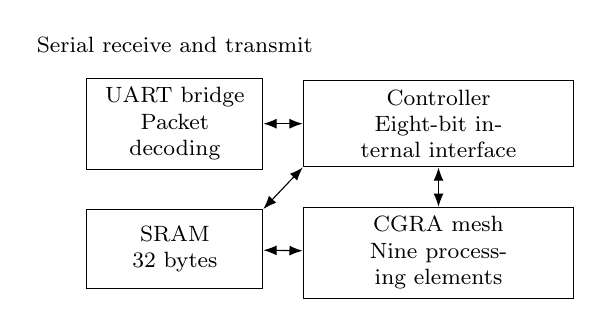
\begin{tikzpicture}[node distance=5mm,box/.style={draw,align=center,font=\footnotesize,minimum height=10mm},>=Latex]
\node[box,text width=2cm] (uart) {UART bridge\\Packet decoding};
\node[box,text width=3.2cm,right=of uart] (ctrl) {Controller\\Eight-bit internal interface};
\node[box,text width=2cm,below=of uart] (sram) {SRAM\\32 bytes};
\node[box,text width=3.2cm,below=of ctrl] (array) {CGRA mesh\\Nine processing elements};
\draw[<->] (uart)--(ctrl);
\draw[<->] (ctrl)--(array);
\draw[<->] (ctrl.south west)--(sram.north east);
\draw[<->] (sram)--(array);
\node[font=\footnotesize,above=2mm of uart] {Serial receive and transmit};
\end{tikzpicture}
\caption{NanoCGRA application-level organization. The UART interface provides the four-signal boundary used by the padframe configuration. Clock and reset are shared.}
\label{fig:nano}
\end{figure}

An independent Python model generates 192 operand pairs, comprising 24 pairs for each of addition, subtraction, AND, OR, exclusive-or, multiplication, multiply--accumulate (MAC), and pass-through. Each operation uses eight boundary pairs and 16 pseudorandom pairs with seed 20261011. Results wrap to eight bits. Configuration loading clears the MAC accumulator, so the MAC cases check a single product, not accumulation across runs. A separate sweep writes and reads all 32 SRAM addresses. The output is PE00, so these tests do not establish coverage of all mesh routes.

The testbench transmits actual UART bits and checks returned bytes at a 100 ns clock period. It runs with both the accelerated eight-clock divisor and the hardware's default 87-clock divisor. Each measured result includes six three-byte writes, a run packet, a 200-cycle host wait, a read packet, and the returned byte. Latency begins at the first operand-write start bit and ends at completion of that byte. Core latency is measured separately from accepted start to result commit. The testbench asserts both arithmetic agreement and five-cycle core latency for every vector. The scripts, vectors, logs, and per-vector timestamps are retained in the paper workspace.

\subsection{Execution and Provenance}
The experiment copies optimized NanoCGRA RTL and testbenches at repository revision \texttt{4f20f65} into a separate workspace. The original smoke-test verdicts are adapted to the runner and waveform recording is added without changing RTL. Independent performance tests use the same copied RTL. No design is regenerated through an LLM.

The fresh hardening attempt uses LibreLane 3.0.7 and Python-enabled Yosys bindings version 0.66, matching the project's pinned synthesis dependencies. It selects GF180MCU-D, the seven-track \texttt{gf180mcu\_fd\_sc\_mcu7t5v0} library, a 5 V nominal supply, and a 100 ns clock. The installed PDK revision is \texttt{bdc9412b}. Nominal, slow, and fast timing libraries are configured. OpenSTA 2.5.0 is the installed timing executable.

Padframe assembly is executed separately using the retained optimized-core GDSII and DEF. Those files were produced by an earlier physical run, so its timing and cell-count metrics remain historical results. The new assembly uses the repository's bundled \texttt{RING\_PAD.gds}. KLayout reads the generated chip hierarchy and captures the full-layout screenshot. Reports identify both the reused core input and the newly generated assembly output.

To reproduce, run \texttt{paper/measure\_nanocgra.py} for independent UART checks and timestamp extraction. Run \texttt{paper/run\_nanocgra\_e2e.sh} for backend checks and hardening. Then execute \texttt{paper/assemble\_retained\_nanocgra.py} with the recorded retained core GDSII/DEF and \texttt{gf180-v1}. Preserve reports and raw logs for each attempt. The physical failure remains distinct from the retained-core assembly.

\section{Results}
\subsection{Functional Checks and Synthesis}
The original four UART smoke checks pass. The independent expanded test passes 192 arithmetic checks and 32 SRAM checks at each of two UART divisors, giving 448 passing checks. All eight operations agree with the Python model, and every tested computation commits five cycles after accepted start. This is measured RTL behavior, not exhaustive state-space verification or silicon measurement.

Icarus syntax and elaboration checking passes. The hardening flow's Verilator stage reports 298 warnings, so this run is not described as warning-free lint. Fresh synthesis completes with $129{,}736.32\,\mu$m$^2$ of mapped cell area, of which $39{,}278.71\,\mu$m$^2$ is sequential logic. These values describe the newly synthesized netlist. They are not substituted for the earlier core implementation's area or timing metrics.

Fresh hardening stops before placement because OpenSTA 2.5.0 lacks a clock property required by LibreLane. A local reporting-flag adaptation resolves an earlier command mismatch, but the property failure remains. Thus no fresh routed core or physical signoff is produced.

\subsection{Measured Latency and Throughput}
Table~\ref{tab:performance} separates core time from serial transaction time. With clock frequency $f$ and measured core cycle count $N$, core latency is $N/f=0.5\,\mu$s. Sequential throughput is
\begin{equation}
R_{\mathrm{seq}}=1/T_{\mathrm{transaction}},
\end{equation}
where $T_{\mathrm{transaction}}$ includes configuration, operands, command spacing, the fixed host wait, and returned data. It describes this reproducible host protocol, not peak array operations per second or overlapped streaming capacity.

\begin{table}[t]
\caption{Measured RTL Performance at 10 MHz}
\label{tab:performance}\centering\footnotesize
\begin{tabular}{lrr}\toprule
Metric & Divisor 8 & Divisor 87\\\midrule
UART rate (kbaud) & 1250.00 & 114.94\\
Core latency (cycles) & 5 & 5\\
Core latency ($\mu$s) & 0.50 & 0.50\\
Full transaction ($\mu$s) & 239.50 & 2392.10\\
RUN through returned result ($\mu$s) & 81.10 & 669.50\\
READ through returned byte ($\mu$s) & 34.80 & 362.50\\
Sequential results per second & 4175.37 & 418.04\\
Passing arithmetic / SRAM checks & 192 / 32 & 192 / 32\\\bottomrule
\end{tabular}
\end{table}

For each divisor, minimum, mean, and maximum transaction times are identical across all 192 vectors because the host schedule and arithmetic pipeline are fixed. The default setting is the representative hardware configuration. Divisor 8 accelerates simulation and is not a measured device baud capability. Serialization dominates the five-cycle core computation. The eight-bit, start/stop-bit UART framing gives a raw byte-rate upper bound of $f/(10C)$ for divisor $C$, before command overhead and host gaps. End-to-end throughput is therefore much lower than this framing bound. Different workloads and interfaces in Table~\ref{tab:related} prevent a defensible numerical speedup comparison.

\subsection{Core Interface Tradeoff}
The retained optimized-core comparison records a reduction from 39 parallel-interface signals to four serial-interface signals. This is an 89.7\% reduction in top-level signal count, excluding power pads and unused ring resources. It comes with an increase from 5,082 to 5,296 synthesized cells and from 116,523 to 123,634 $\mu$m$^2$ of mapped area, approximately 4.2\% and 6.1\%, respectively. The bridge trades serialization latency and additional logic for a smaller external signal interface.

The retained physical report targets 10 MHz and records $+76.72$ ns setup slack and $+0.82$ ns hold slack. Its LVS summary reports 5,325 matched devices and 96 matched cell subcircuits, but also records a residual UART boundary alias. We retain the device/subcircuit agreement without promoting it to an unambiguous full-chip connectivity verdict. These historical results motivate the compatible core chosen for assembly and are distinct from the fresh synthesis attempt.

\subsection{Executed Padframe Assembly}
The new assembly generates a 23,538,006-byte binary GDSII file. Table~\ref{tab:assembly} records its geometry and hierarchy. KLayout independently reads one chip top with direct references to \texttt{RING\_PAD} and \texttt{NanoCGRA\_Lite}. The core translation is $(1254.523,1254.523)\,\mu$m, consistent with the center-offset calculation in (\ref{eq:translation}). The 993 merged entries are GDS cell definitions, not the number of placed standard-cell instances.

\begin{table}[t]
\caption{New Assembly of the Retained NanoCGRA Core}
\label{tab:assembly}\centering\small
\begin{tabular}{ll}\toprule
Metric & Recorded result\\\midrule
Core bounding box & $466.555\times466.555\,\mu$m\\
Ring and chip extents & $2935\times2935\,\mu$m\\
Chip envelope area & $8.614225$ mm$^2$\\
Configured I/O resources & 69 pads and four corners\\
Merged cell definitions & 993\\
Signal routes & Four on Metal2\\
Supply routes & Seven on Metal3\\
Direct chip instances & Ring and translated core\\\bottomrule
\end{tabular}
\end{table}

\begin{figure}[t]
\centering
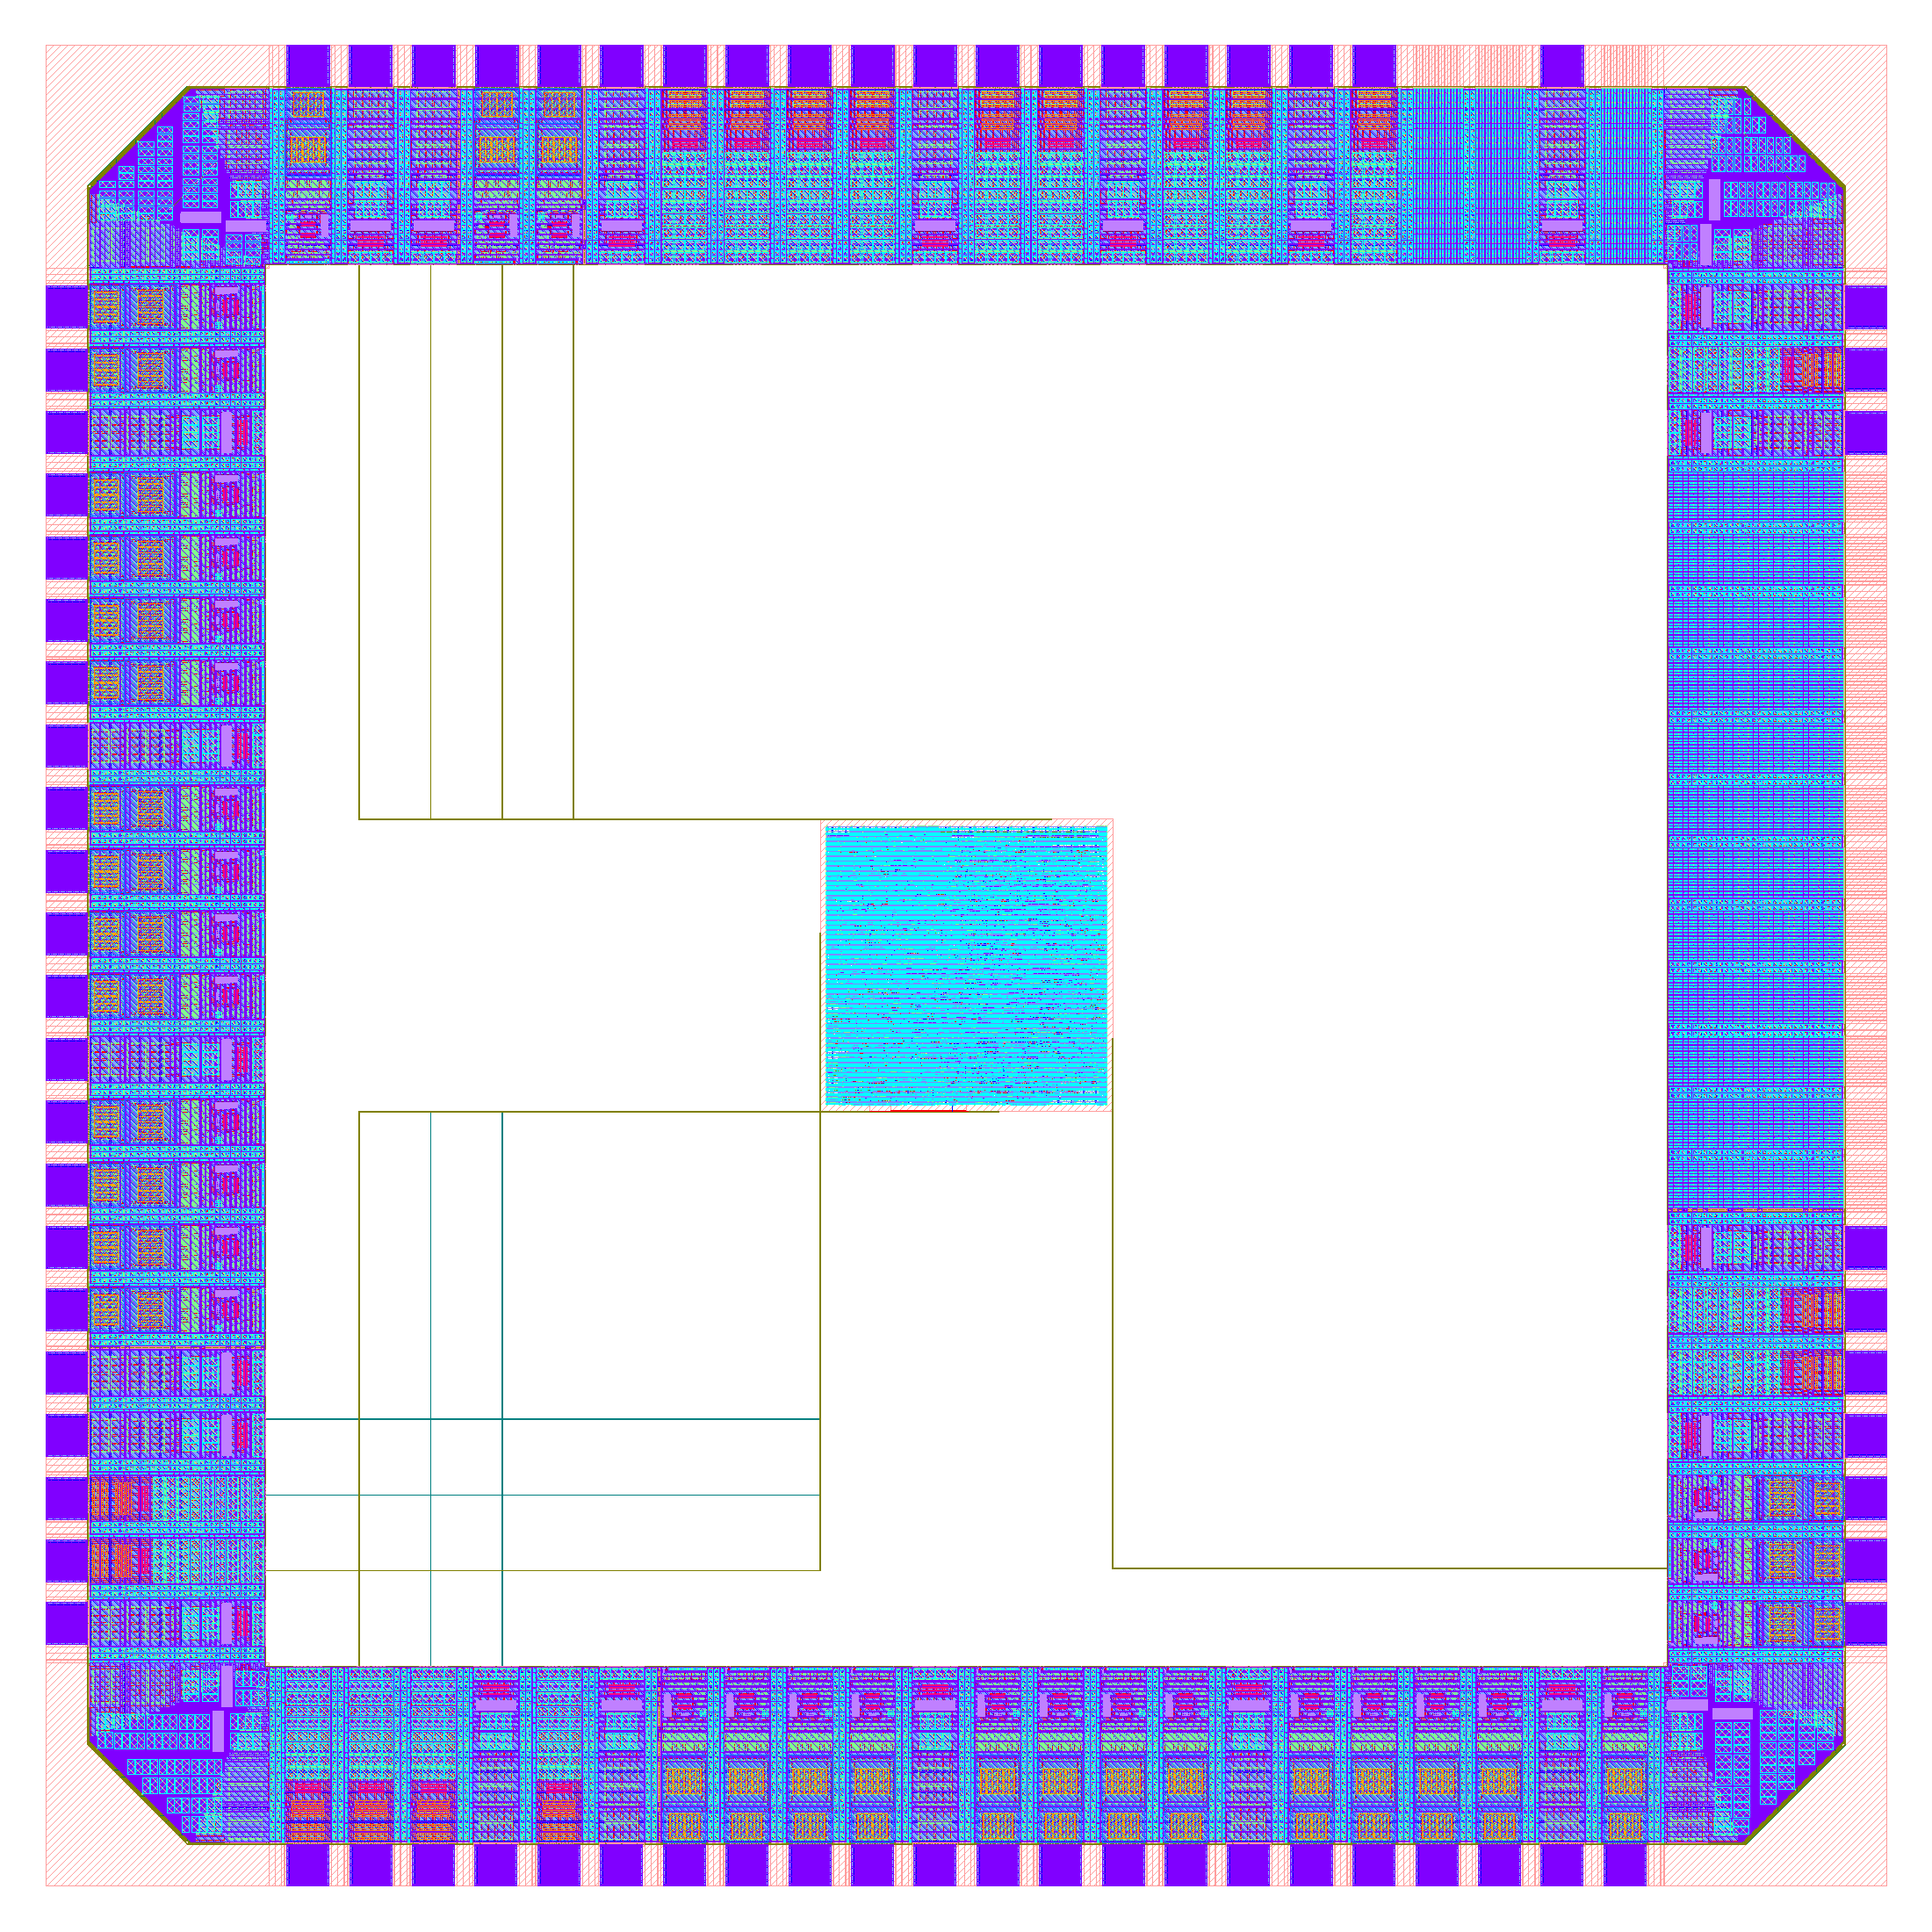
\includegraphics[width=3.3in]{figures/nanocgra_padframe_klayout.png}
\caption{KLayout screenshot of the generated NanoCGRA chip GDSII. The 2.935 mm square reusable ring surrounds the retained 466.555 $\mu$m square core. The visible pad-to-core routes are geometric assembly results, with full-chip electrical verification pending.}
\label{fig:padframe}
\end{figure}

Fig.~\ref{fig:padframe} shows the assembled GDSII with full hierarchy visible. Four signal routes connect clock, reset, receive, and transmit geometry. Three supply and four ground resources produce seven supply routes. Independent readback establishes that these shapes coexist with the ring and core.

The core bounding box occupies approximately 2.53\% of the chip envelope. This is a geometric footprint ratio, not standard-cell utilization. The fixed ring dominates area, so fewer signals do not demonstrate a smaller package.

\section{Discussion and Limitations}
\subsection{Acceptance at the Chip Boundary}
Hierarchy readback establishes a readable layout containing the selected blocks. Estimated routing endpoints may miss pins or need vias and orientation transforms. Electrical continuity requires full-chip LVS against a complete core and I/O-cell netlist.

Full-chip DRC must check new routes, supply continuity, voltage compatibility, unused-pad ties, and keep-out regions. The demonstrated assembly therefore remains short of electrically verified, fabrication-ready integration.

\subsection{Scope of the Platform Evaluation}
The experiment demonstrates backend execution, fresh RTL checks and synthesis, and retained-core assembly. It does not evaluate LLM generation, reference approval, scheduling, or autonomous repair. Engineering-effort reduction, multi-seed completion rate, and portability remain unmeasured. The hardening failure makes compatible tool versions part of the reproduction contract.

Future work should test broader mesh configurations, UART faults, accumulated MAC sequences, and deliberate connectivity errors. A scripted baseline should measure completion rate, interventions, runtime, and cost. Compatible implementation tools, pin-accurate routing, and full-chip DRC/LVS are immediate priorities before fabrication and power measurement.

\section{Conclusion}
Chip Orchestra preserves evidence across hardware-generation and implementation stages. NanoCGRA passes 448 UART checks at two serial settings with five-cycle core latency. Fresh synthesis completes, and a separate execution assembles a retained core into a 2.935 mm square ring. The GDSII screenshot and hierarchy readback demonstrate assembly. Compatible hardening tools and full-chip electrical verification remain necessary for a completed chip implementation.

\clearpage
\begin{thebibliography}{11}
\bibitem{openroad} The OpenROAD Project, ``OpenROAD documentation.'' Accessed Oct. 11, 2026. [Online]. Available: \url{https://openroad.readthedocs.io/en/latest/}
\bibitem{librelane} LibreLane Contributors, ``LibreLane documentation.'' Accessed Oct. 11, 2026. [Online]. Available: \url{https://librelane.readthedocs.io/en/latest/}
\bibitem{chipgpt} K. Chang et al., ``ChipGPT: How far are we from natural language hardware design,'' 2023, arXiv:2305.14019v1.
\bibitem{autochip} S. Thakur et al., ``AutoChip: Automating HDL generation using LLM feedback,'' 2024, arXiv:2311.04887v2.
\bibitem{rtllm} Y. Lu, S. Liu, Q. Zhang, and Z. Xie, ``RTLLM: An open-source benchmark for design RTL generation with large language model,'' in \emph{Proc. ASP-DAC}, 2024, arXiv:2308.05345.
\bibitem{verilogeval} M. Liu, N. Pinckney, B. Khailany, and H. Ren, ``VerilogEval: Evaluating large language models for Verilog code generation,'' in \emph{Proc. ICCAD}, 2023, arXiv:2309.07544v2.
\bibitem{chipchat} J. Blocklove, S. Garg, R. Karri, and H. Pearce, ``Chip-Chat: Challenges and opportunities in conversational hardware design,'' in \emph{Proc. MLCAD}, 2023, doi: 10.1109/MLCAD58807.2023.10299874.
\bibitem{chateda} H. Wu et al., ``ChatEDA: A large language model powered autonomous agent for EDA,'' \emph{IEEE Trans. Comput.-Aided Design Integr. Circuits Syst.}, 2024, doi: 10.1109/TCAD.2024.3383347.
\bibitem{opencgra} C. Tan, C. Xie, A. Li, K. J. Barker, and A. Tumeo, ``OpenCGRA: An open-source unified framework for modeling, testing, and evaluating CGRAs,'' in \emph{Proc. ICCD}, 2020, pp. 381--388, doi: 10.1109/ICCD50377.2020.00070.
\bibitem{morpher} D. Wijerathne, Z. Li, and T. Mitra, ``Accelerating edge AI with Morpher: An integrated design, compilation and simulation framework for CGRAs,'' in \emph{Proc. CODAI}, 2023, arXiv:2309.06127.
\bibitem{gf180} GlobalFoundries PDK Authors, ``GF180MCU PDK documentation,'' 2022. Accessed Oct. 11, 2026. [Online]. Available: \url{https://gf180mcu-pdk.readthedocs.io/en/latest/}
\end{thebibliography}
\end{document}
